\documentclass[12pt]{article}

\usepackage{geometry}
\usepackage{graphicx}
\usepackage{tabularx}
\usepackage{caption}
\usepackage{xcolor}
\usepackage{hyperref}
\hypersetup{
    colorlinks=false,
    linkbordercolor=red,
    urlbordercolor=blue,
    pdfborder={1 1 1},
    pdfborderstyle={/S/U/W 1}
}
\usepackage[indent=0pt]{parskip}

\geometry{
a4paper,
left=3cm,
right=3cm,
top=3cm,
bottom=3cm }

\author{Silvio d'Antonio, Riccardo Mearelli, Carlo Segreto}
\date{\today}
\title{Visual Analytics Project Proposal}

\begin{document}

\maketitle

\section{General idea}

We are proposing to develop a visualization system with the purpose of
providing general insights on the topic of vehicle accidents in Italy.

\subsection*{Intended users}

The intended users for this system would be members of the Ministry of
Transport, police and traffic authorities, helping them with taking informed decision on how to better prevent
accidents in Italy, particularly those involving injuries.

\section{Dataset}

The dataset contains details about vehicle accidents with injuries
occurred in Italy during 2024. This dataset was extracted from the data
published on the
\href{https://esploradati.istat.it/databrowser/#/en/dw/categories/IT1,Z0810HEA,1.0/HEA_ROAD/IT1,41_269_DF_DCIS_INCIDENTISTR1_1,1.0}{ISTAT website}
and comprises about 92.000 tuples, each described by 8 attributes.

The attributes in the dataset are in summary: region and time (hour, weekday,
month) of accident, road section where the accident occurred (traffic circle,
intersection, etc...), type of accident (between vehicles, vehicle-pedestrian,
etc...), deadliness of the accident, and number of accidents registered with
the given characteristics.

More details are provided with a table at the end of the proposal.

\section{Visualization System Description}

\begin{figure}[!ht]
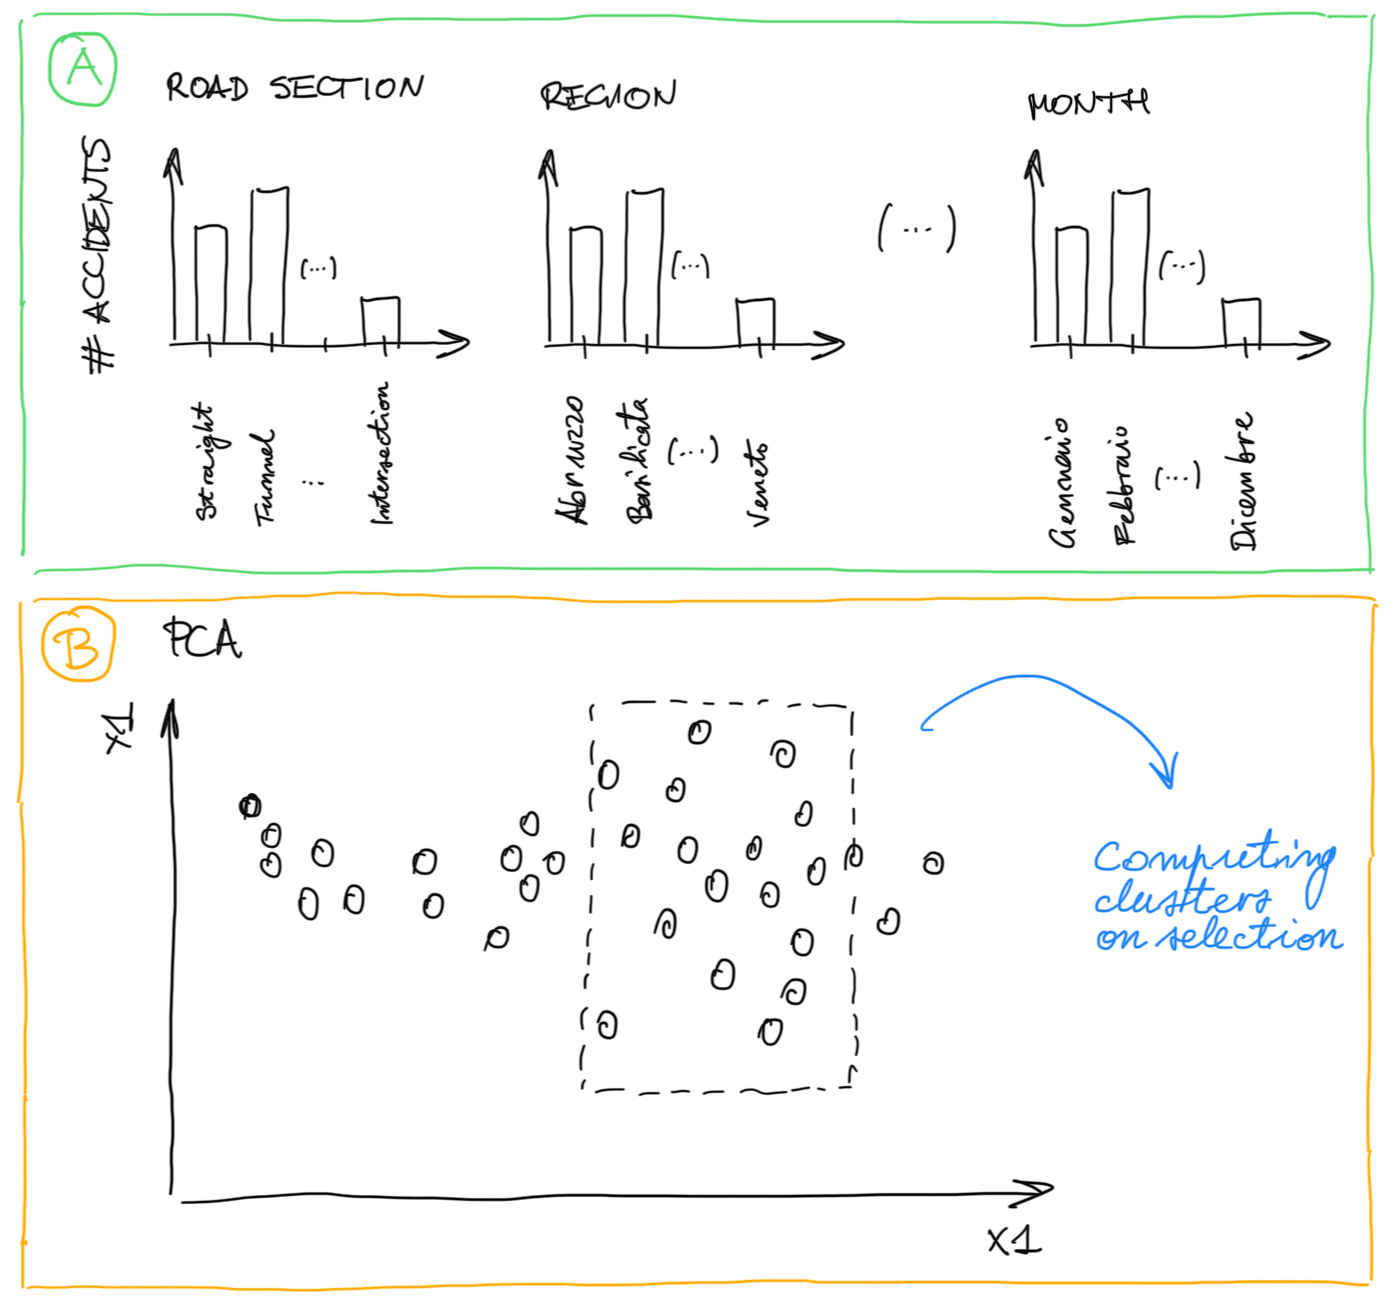
\includegraphics[width=1\linewidth]{draft.jpg}
\caption{Draft of the visualization system.}
\label{fig:draft}
\end{figure}

The system is composed of two main sections as shown in Figure \ref{fig:draft}.

Section A visualizes the number of accidents for each main attribute
of the dataset. This is is done through different bar charts with categorical values displayed along the horizontal axis (X) and the number of accidents along the vertical axis (Y).
These charts are coordinated with each other.
As an example, selecting the accidents that occurred between January and March
also highlights the corresponding road section types and accident categories within that timeframe.


Section B presents the result of a PCA performed on the dataset.
Data points can be colored according to the categorical attributes of the dataset:
accident type, deadliness etc.
The PCA graph is coordinated with the charts in section A.
As an example, selecting accidents that occurred between January and March in Section A highlights the corresponding data points in the PCA plot, and vice versa.

Furthermore, the user can visually trigger an analytic directly brushing on the PCA graph, the system will respond by searching for clusters (\textit{e.g. with k-means}) within the selected subset of data points.



\section{Dataset Details}

\begin{tabularx}{\textwidth} {| >{\bfseries}l | X |} 

\hline
Attribute & \textbf{Description} \\
\hline\hline

Area & ID of Region \\
\hline
Road section & Number identifying a road section. Identifies: tunnel, bend, crossroad, traffic circle, bump/slope or bottleneck, straight stretch, level crossing. \\
\hline
Accident type &  Number identifying the accident type. Identifies:
accidents between vehicles, vehicle-pedestrian accidents and accidents involving
a single vehicle. \\ 
\hline
Deadliness &  Boolean attribute that identifies if the accident involved death or only injury \\
\hline
Hour of accident &  Time of accident measured with hour resolution \\
\hline
Month &  Month number \\
\hline
Weekday & Number identifying the weekdays: monday, tuesday, wednesday, etc...\\
\hline
Observations &  Number of accidents occurred with the specified attributes \\
\hline
\end{tabularx}

\end{document}
